\documentclass[deposito, acronym, symbols]{fei}

%\usepackage{glossaries}
\usepackage{subcaption} 
\usepackage{graphicx}
\usepackage{float}
%\usepackage{units}
\usepackage[portuguese]{algorithm2e}
\usepackage{biblatex}
\usepackage{amsmath}
\usepackage{listings}
\usepackage[utf8]{inputenc}
\usepackage{chngcntr} %Faz com que o numero das notas de rodape aumente crescentemente.
\usepackage{appendix}
\counterwithout{footnote}{chapter}% "
\usepackage{siunitx}
\sisetup{output-exponent-marker=\ensuremath{\mathrm{e}}} %Escrita que precede cada entrada na lista de ilustrações.
\renewcommand{\cftfigurepresnum}{Figura }
\setlength{\cftfigurenumwidth}{5.7em}

\usepackage{titling}

%\makeglossaries
%%\newacronym[] {achpt} {ACT} {Aparecido ChupeTão}

\newacronym[longplural=Associações Brasileiras de Normas Técnicas]{abnt}{ABNT}{Associação Brasileira de Normas Técnicas}

\newacronym{ibge}{IBGE}{Instituto Brasileiro de Geografia e Estatística}

\newacronym{ashrae}{ASHRAE}{\textit{American Society of Heating, Refrigerating and Air-Conditioning Engineers}}

\newacronym{nbr}{NBR}{Norma Brasileira}

\newacronym{pmv}{PMV}{\textit{Predicted Mean Vote}}
	
\newacronym{ppd}{PPD}{\textit{Predicted Percentage of Dissatisfied}}
		
\newacronym{vgd}{VGD}{Ventilação Geral Diluidor}
		
\newacronym{vgl}{VGL}{Ventilação Local Exaustora}
		
\newacronym{cfd}{CFD}{\textit{Computational Fluid Dynamics}}
		
\newacronym{pcb}{PCB}{\textit{Printed Circuit Board}}
		
\newacronym{sms}{SMS}{\textit{Short Message Service}}
		
%\newglossaryentry{pi}{parent=greek,type=symbols,name={\ensuremath{\pi}},sort=p,description={número irracional que representa [razão entre a circunferência de qualquer círculo e seu diâmetro]}}
		


\title{Relatório da Atividade A4 - Grupo D}
\author{Ana Sung Marques \\Felipe Estevão Coquito de Mello\\  Gabriel de Souza Simonetti  \\ Gabriel Mola da Silva \\ Netuno Trindade Torrente Rovaroto \\ Victor Salzo Lopes  \\ Vitoria Fedatto Stefaneli}
\cidade{São Bernardo do Campo}
\instituicao{Centro Universitário FEI}

\addbibresource{Referencias.bib}
%\bibliographystyle{plain}
\bibliography{Referencias}
\graphicspath{ {Imagens/}, {Tabelas/}}

\begin{document}
\maketitle

\begin{folhaderosto}
	Trabalho de Conclusão de Curso apresentado ao Centro Universitário FEI, como parte dos requisitos necessários para obtenção do título de Bacharel em Engenharia Mecânica. Orientado pelo Prof. Cyro Albuquerque Neto.
\end{folhaderosto}

\listoffigures


\chapter{Introdução}

Partindo do modelo 3D da retroescavadeira, analisado no software Ansys, foi realizado a montagem do protótipo da estrutura. Durante esta fase, foram realizados, também, os testes da estrutura, para garantir de que tudo esteja de acordo com as requisições do projeto.

\chapter{Estágio Atual de Desenvolvimento do Projeto}

Conforme apresentado anteriormente, após o Brainstorming e o Funil de ideias, o grupo optou pela combinação das ideias, utilizando especificamente a base de funcionamento de uma impressora 3D (Figura \ref{fig: Impressora 3D}), combinado com o mecanismo de acionamento de uma retroescavadeira clássica (Figura \ref{fig: Escavadeira Manal do Mundo}).

\begin{figure}[!htp]
  \centering
  \begin{minipage}{0.4\textwidth}
        \caption{Representação dos movimentos de uma impressora 3D}
        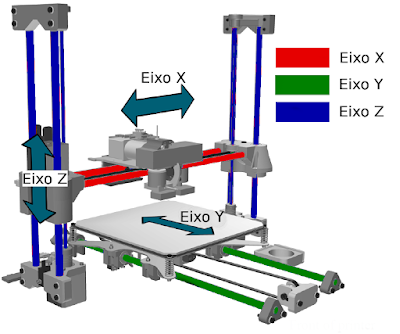
\includegraphics[width=0.65\linewidth]{Imagens/Impressora 3D.png}
        \smallcaption{Disponivel em: <http://3drecycler.blogspot.com/2018/04/como-funciona-uma-impressora-3d.html>}
        \label{fig: Impressora 3D}
  \end{minipage}
  \hfill
  \begin{minipage}{0.4\textwidth}
        \caption{Exemplo de escavadeira hidráulica produzida a partir de seringas}
        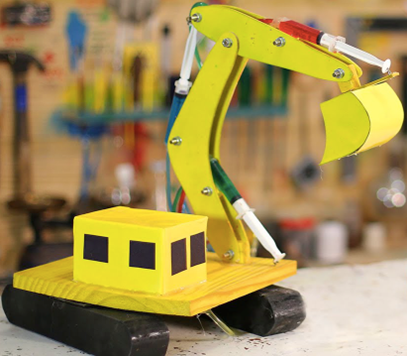
\includegraphics[width=0.65\linewidth]{Imagens/Manual do mundo.png}
        \smallcaption{Disponivel em: <https://www.youtube.com/watch?v=e83drbSOoi4>}
        \label{fig: Escavadeira Manal do Mundo}
  \end{minipage}
\end{figure}

A ideia do grupo foi desenvolver uma série de trilhos onde a lança da escavadeira consegue se locomover livremente no sentido X e Y com o auxílio de rodas acopladas. Para a movimentação no eixo Z foi pensado no uso de um molinete, liberando a garra para o movimento de descida e subida. Referente ao movimento de rotação da garra, o grupo pensou no uso de uma seringa para fazer o trabalho de um pistão hidráulico.


Ultilizando software Autodesk Inventor, foi realizada a modelagem do protótipo 3D, Figura [\ref{fig: Prototipo}]. Em posse do desenho da estrutura, analisado o mesmo no software Ansys, verificou-se a estabilidade da estrutra, viabilizando o corte a laser das peças em MDF. Para isso, utilizou-se os equipamentos do Centro de Laboratório Mecânico do Centro Universitário FEI.

 \begin{figure}[!htb]
 \centering
    \caption{Desenho 3D do Protótipo}
    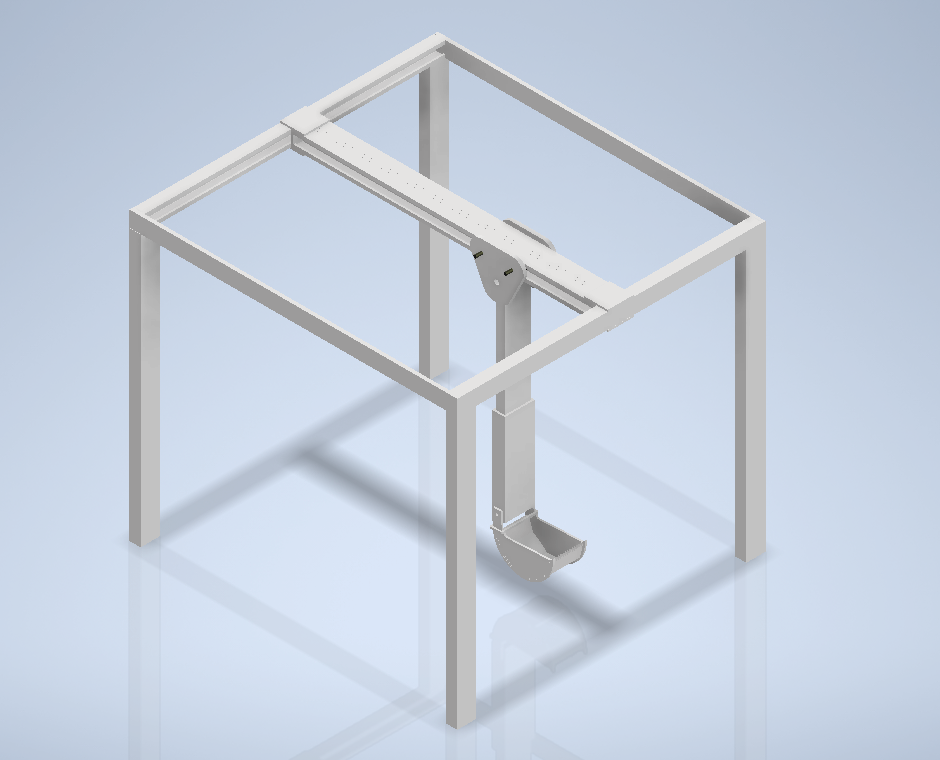
\includegraphics[width=1\linewidth]{Imagens/Prototipo.png}
    \smallcaption{Fonte: Autor}
    \label{fig: Prototipo}
 \end{figure}

\chapter{Protótipo em escala reduzida}

Após o desenvolvimento da representação 3D da retroescavadeira, as peças foram cortadas a laser no Centro de Laboratórios Mecânicos (CLM) da FEI e a montagem do protótipo foi iniciada. Vale ressaltar que utilizou-se chapas de MDF de espessuras 3mm e 6mm para o corte a laser e os componentes foram unidos a partir de cola branca, exceto os eixos, para os quais utilizou-se cola quente.

  \begin{figure}[!htb]
 \centering
    \caption{Montagem do Protótipo - Composição da garra e seu sistema de movimentação}
    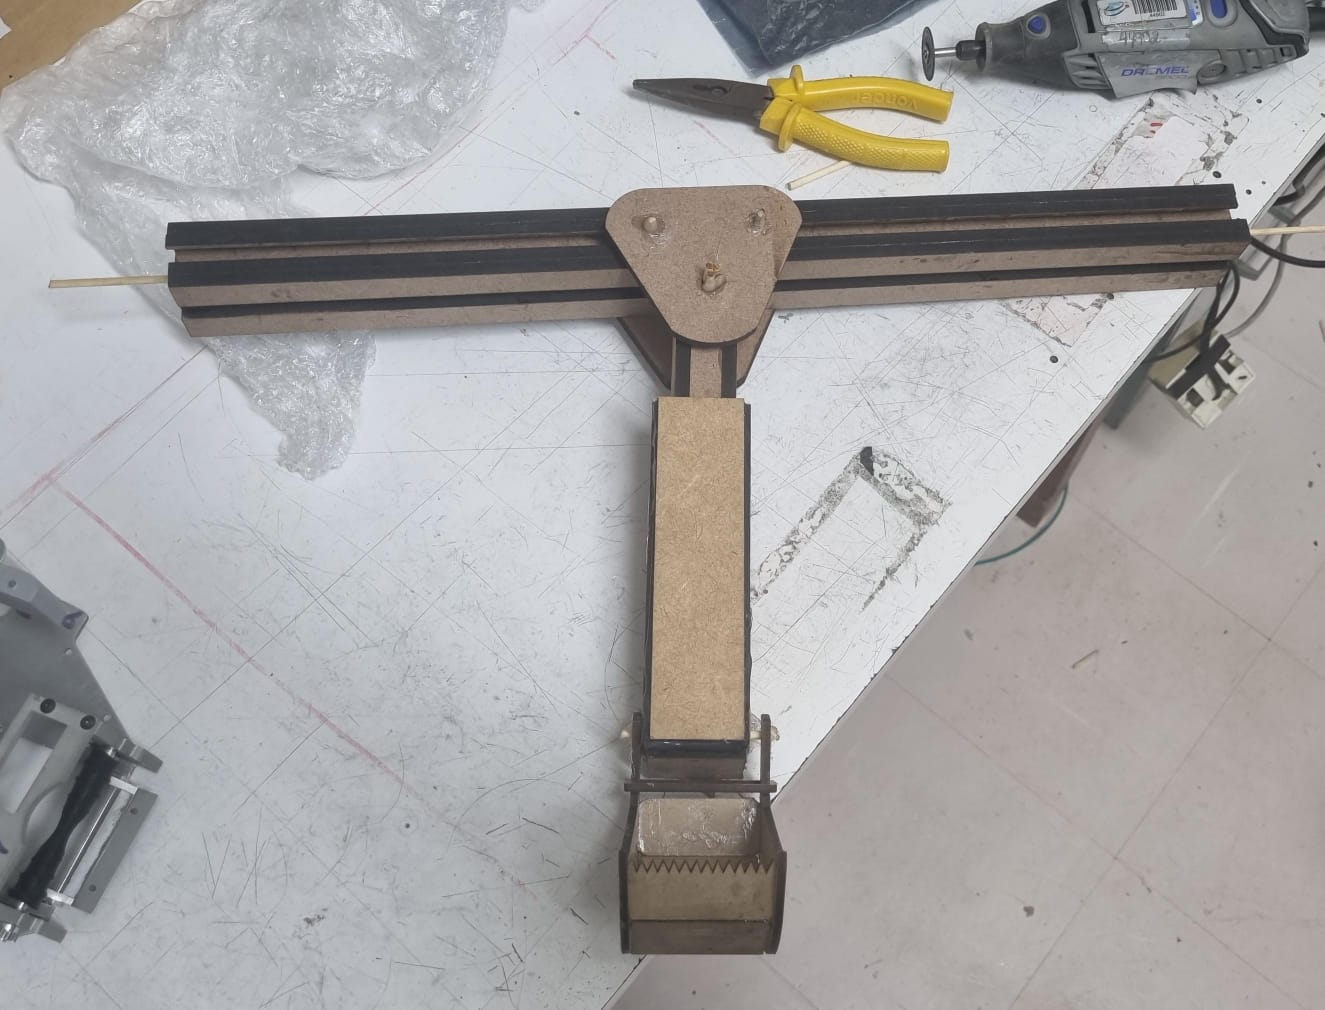
\includegraphics[width=0.8\linewidth]{Imagens/GARRA.jpeg}
    \smallcaption{Fonte: Autor}
    \label{fig: 2D-3_1}
 \end{figure}
 
  \begin{figure}[!htb]
 \centering
    \caption{Montagem do Protótipo - Sistema de movimentação da estrutura partindo de rodas de MDF}
    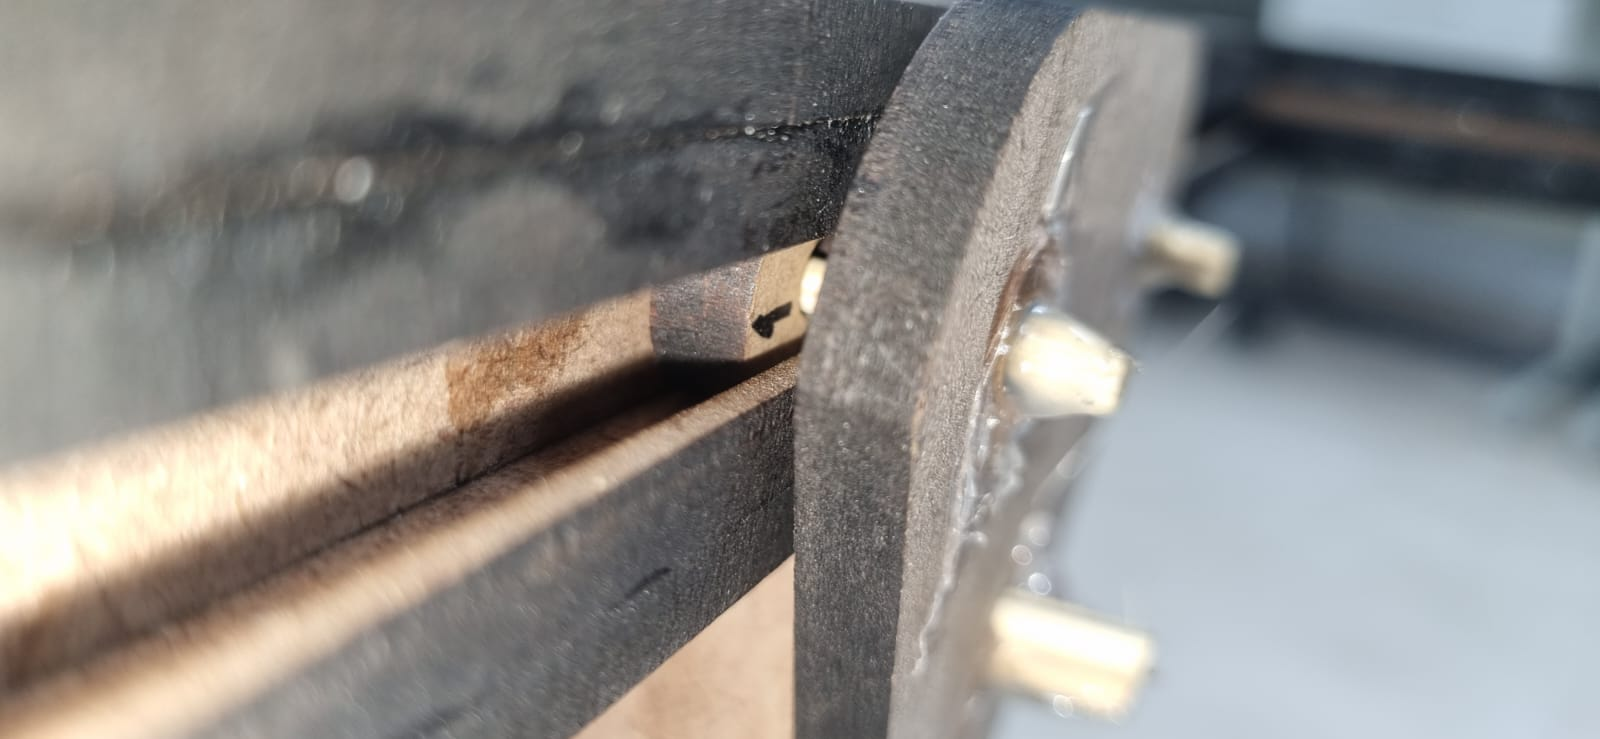
\includegraphics[width=0.7\linewidth]{Imagens/ROLAMENTO.jpeg}
    \smallcaption{Fonte: Autor}
    \label{fig: 2D_6_1}
 \end{figure}
 
O componete do protótipo, Figura \ref{fig: 2D-3_1} é responsável pela movimentação horizontal da garrra, composta por dois trilhos simétricos adjacentes entre si, a movimentação é composta por 2 rodas por trilho e são unidas por 2 chapas de MDF, Figura  \ref{fig: 2D_6_1}, onde através dos eixos se conectam ao módulo da garra.

   \begin{figure}[!htb]
 \centering
    \caption{Montagem do Protótipo - Garra inserida na estrutura de pórtico}
    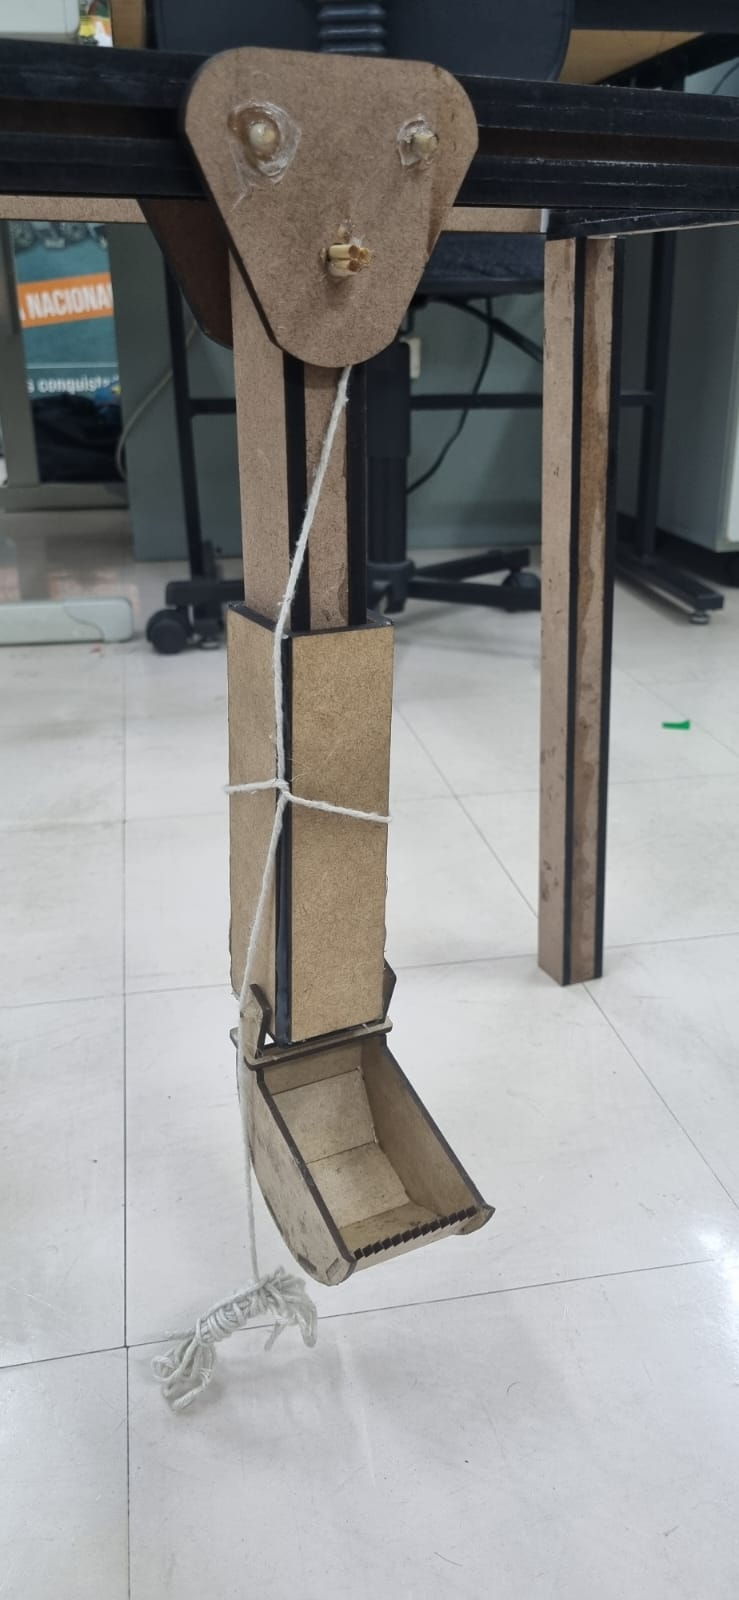
\includegraphics[width=0.5\linewidth]{Imagens/GARRA MONTADA.jpeg}
    \smallcaption{Fonte: Autor}
    \label{fig: 2D_3_2}
 \end{figure}

O módulo da garra, Figura \ref{fig: 2D_3_2}, é composto por dois paralelepípedos e a pá da escavadeira, este módulo é responsável pelo movimento de extenção da pá, através da diferença de altura dos dois paralelepípedos e regulagem com fio.

  \begin{figure}[!htb]
 \centering
    \caption{Montagem do Protótipo - Estrutura inicial}
    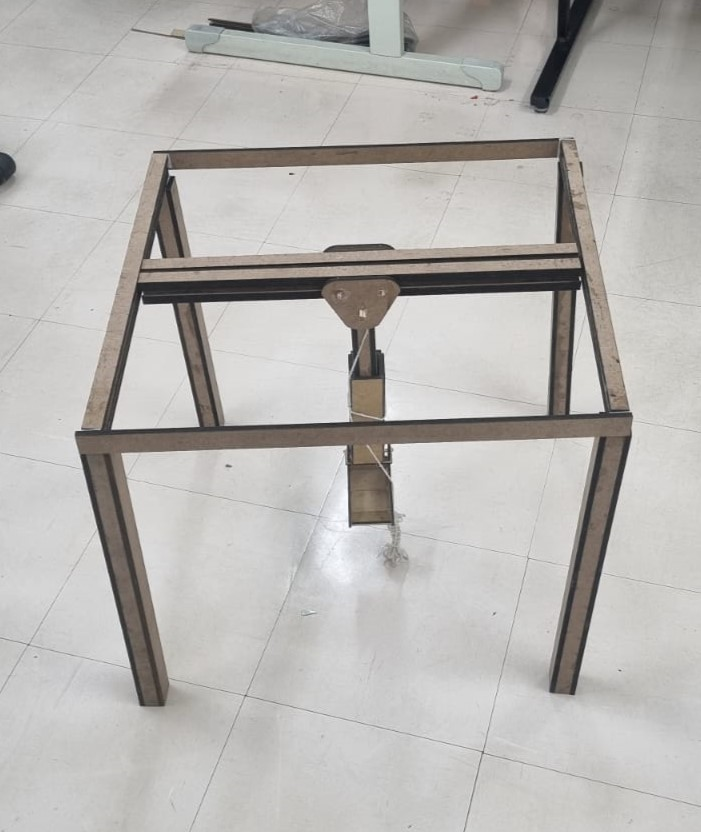
\includegraphics[width=0.8\linewidth]{Imagens/GARRA CERTA.jpeg}
    \smallcaption{Fonte: Autor}
    \label{fig: 2D_6_2}
 \end{figure}

Colando os pés e as laterais, responsáveis pela movimentação no eixo Y, temos o protótipo completo do sistema, Figura \ref{fig: 2D_6_2}.

Após a montagem, os testes foram efetuados e estão disponíveis para visualização em: \url{https://youtu.be/xOaCKu2gUXc?si=hDwvoQIrM8m4ORZY}

\chapter{Simulações estruturais}
 
Como  citado anteriormente, foi utilizado o software ANSYS para a realização das simulações estruturais, mais especificamente a opção de “Static Structural”, pela estrutura assemelhar-se a uma espécie de Pórtico estático.

\section{Planejamento}

O grupo optou por fazer tal análise no software ANSYS, para que fosse possível validar sua integridade em funcionamento e até mesmo verificar se não haveria nenhum tipo de mal dimensionamento por parte das peças, materias ou desenho, como a necessidade de uma parede mais espessa por exemplo. 

\section{Geométrica}

O primeiro passo foi realizar um upload no software ANSYS do modelo 3D, citado anteriormente, e verificar se havia algum defeito ou erro no mesmo. Abaixo está indicado o modelo 3D no software ANSYS: Figura [\ref{fig: geometry}].

 \begin{figure}[!htb]
 \centering
    \caption{Geometrica no Ansys}
    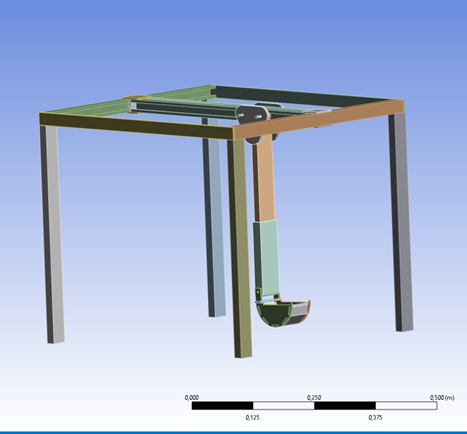
\includegraphics[width=0.75\linewidth]{Imagens/Geometria.png}
    \smallcaption{Fonte: Autor}
    \label{fig: geometry}
 \end{figure}

\newpage

\section{Materiais}

 Foi escolhido o compensado de MDF de diferentes espessuras por se tratar de um material já disponível pela faculdade, sendo elas 6mm para as fixações, estrutura do suposto pórtico e rodas, e 3mm para garra e partes móveis da retroescavadeira.
 Após pesquisas, aferiu-se as propriedades do MDF como presentes na Tabela [\ref{fig: Prop.Mec_MDF (A2)}].

 \begin{figure}[!htb]
 \centering
    \caption{Propriedades Fisico-Mecânicas}
    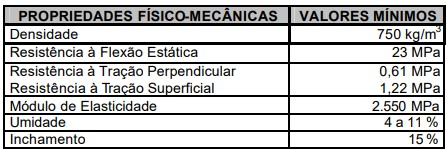
\includegraphics[width=0.75\linewidth]{Imagens/Prop.Mec_MDF (A2).jpg}
    \smallcaption{Fonte: Autor}
    \label{fig: Prop.Mec_MDF (A2)}
 \end{figure}
 
\section{Malha}

Logo após, foi necessário criar uma malha para a estrutura a fim de que o software conseguisse realizar a simulação da forma correta. Vale ressaltar que por uma questão de limitação computacional, não foi possível refinar ao extremo esta malha, se tornando possível concluir que alguns resultados poderiam ser ainda mais verosímeis com uma malha mais refinada.  

Na Figura [\ref{fig: malha}]  está indicado a malha aplicada a estrutura, assim como as dimensões dos elementos desta malha, na Figura [\ref{fig: Referencia de malha 1}].

 \begin{figure}[!htb]
 \centering
    \caption{Representação da Malha}
    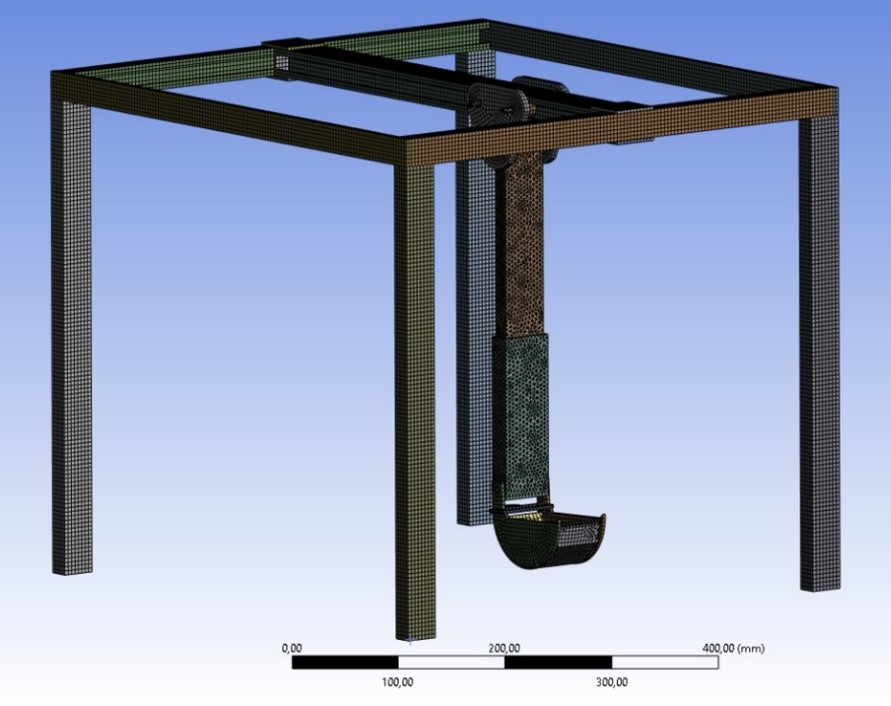
\includegraphics[width=0.7\linewidth]{Imagens/Malha.jpg}
    \smallcaption{Fonte: Autor}
    \label{fig: malha}
 \end{figure}

\begin{figure}[!htp]
  \centering
  \begin{minipage}{0.7\textwidth}
        \caption{Referência da malha}
        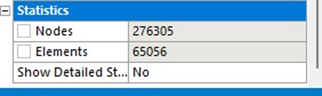
\includegraphics[width=0.65\linewidth]{Imagens/Ref_malha_1.png}
        \label{fig: Referencia de malha 1}
  \end{minipage}
  \hfill
  \begin{minipage}{0.6\textwidth}
        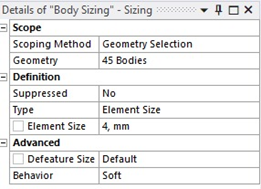
\includegraphics[width=0.6\linewidth]{Imagens/Ref_malha_2.png}
        \smallcaption{Autor}
  \end{minipage}
\end{figure}

\newpage

\section{Contato entre os elementos}

Na sequência se fez necessário aplicar uma ferramenta chamada “Contact Tool”, para verificar quais superfícies não estavam em contato umas com as outras e solucionar este problema. Afinal, se durante a simulação o software encontrasse alguma superfície sem contato com suas respectivas “vizinhas”, o esforço no qual a estrutura está sendo sujeitada não seria transmitido por essas determinadas partes e ocorreria uma falha nos dados encontrados na simulação. 

Por este motivo, se fez necessário criar uma esfera de transmissão de esforços, para que que as partes que estão dentro da área desta esfera, estejam em “contato” e, portanto, realizando a transmissão dos esforços por este determinado local. A Figura [\ref{fig: Esforcos_1}] representa as esferas de transmissão de esforços.


\begin{figure}[!htp]
  \centering
  \begin{minipage}{0.7\textwidth}
        \caption{Imagem das esferas de transmissão de esforços}
        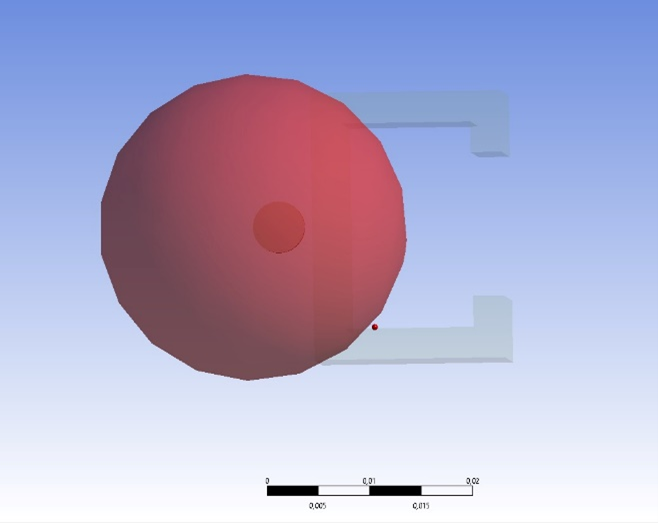
\includegraphics[width=0.65\linewidth]{Imagens/Esforcos_1.png}
        \label{fig: Esforcos_1}
  \end{minipage}
  \hfill
  \begin{minipage}{0.6\textwidth}
        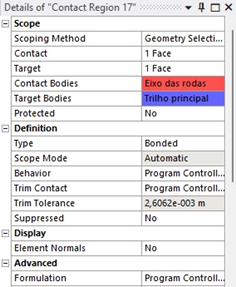
\includegraphics[width=0.6\linewidth]{Imagens/Esforcos_2.png}
        \smallcaption{Autor}
  \end{minipage}
\end{figure}

\newpage
Na Figura  [\ref{fig: Esforcos_1}], nota-se que o eixo de rodas e o trilho principal não estão em contato e como foi supramencionado, isso irá influenciar negativamente no resultado final, por isso foi necessário inserir a esfera de transmissão de esforços, mostrada em vermelho, para indicar ao software o local correto para realizar as devidas transmissões de esforços necessárias.

Após criar todas as esferas necessárias e verificar em uma tabela gerada pelo próprio ANSYS se não havia nenhuma outra parte da estrutura que estivesse fora de contato, seguiu-se com a simulação. Na Figura [\ref{fig: verificação do ANSYS}] é possivel ver a Tabela de verificação do ANSYS.

 \begin{figure}[!htb]
 \centering
    \caption{Tabela de verificação do ANSYS}
    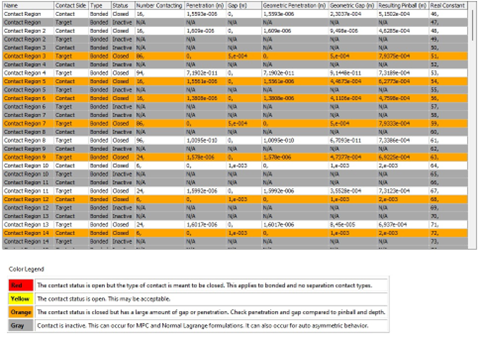
\includegraphics[width=1\linewidth]{Imagens/verificação do ANSYS.png}
    \smallcaption{Fonte: Autor }
    \label{fig: verificação do ANSYS}
 \end{figure}
 
\newpage

\section{Configuração das Análises (Forças e considerações)}

Posteriormente, foi aplicado as forças e parâmetros necessárias, para que o software realizasse a simulação da forma mais verossímil possível.

A principal força foi aplicada na pá da retroescavadeira, que tem valor de 1 N, simbolizando a força peso da massa de areia que será carregada na aplicação prática. Outra força importante que foi levada em conta para a simulação, foi a força da gravidade, afinal, a mesma acaba influenciando diretamente na própria estrutura real, e, portanto, é de suma importância levá-la em consideração. Por último, mas não menos importante, foi fixado os quatro “pés” de estrutura ao solo, considerando que os mesmos permanecerão imóveis durante a simulação e durante a aplicação prática. As Figuras [\ref{fig:foto_força aplicada} \ref{fig:força aplicada_1}] detalha a força aplicada na pá da retroescavadeira e a Figura [\ref{fig:força aplicada_3}] da detalhes da força de gravidade, e do suporte fixo dos “pés”.

 \begin{figure}[!htb]
 \centering
    \caption{Detalhes da força aplicada na pá da retroescavadeira}
    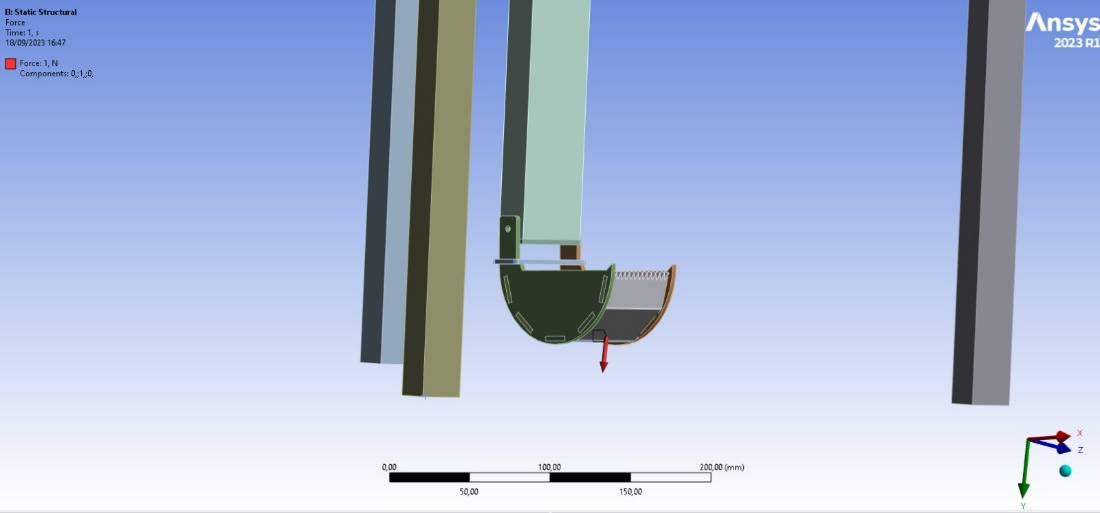
\includegraphics[width=0.8\linewidth]{Imagens/foto_força aplicada.png}
    \smallcaption{Fonte: Autor}
    \label{fig:foto_força aplicada}
 \end{figure}

 \begin{figure}[!htp]
  \centering
  \begin{minipage}{0.6\textwidth}
        \caption{Referência do Structural}
        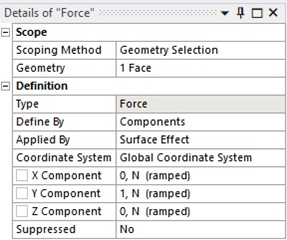
\includegraphics[width=0.65\linewidth]{Imagens/força aplicada_1.png}
        \label{fig:força aplicada_1}
  \end{minipage}
  \hfill
  \begin{minipage}{0.7\textwidth}
        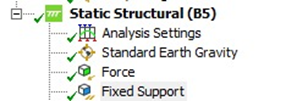
\includegraphics[width=0.6\linewidth]{Imagens/força aplicada _2.png}
        \smallcaption{Autor}
  \end{minipage}
\end{figure}

 \begin{figure}[!htp]
  \centering
  \begin{minipage}{0.7\textwidth}
        \caption{Referência do Global Coordinate}
        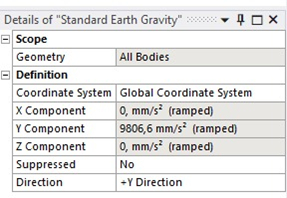
\includegraphics[width=0.6\linewidth]{Imagens/força aplicada_3.png}
        \label{fig:força aplicada_3}
  \end{minipage}
  \hfill
  \begin{minipage}{0.7\textwidth}
        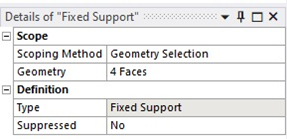
\includegraphics[width=0.6\linewidth]{Imagens/força aplicada_4.png}
        \smallcaption{Autor}
  \end{minipage}
\end{figure}

\newpage

\section{Resultado das soluções}

 Por fim, se fez necessário selecionar os tipos de análises dentre as opções disponíveis, a forma como seria calculado, e rodar a simulação, obtendo os seguintes resultados.

A Deformação total da estrutura, vale ressaltar que a deformação indicada na Figura [\ref{fig:Resultado_1}] é exagerada, para ter uma melhor visualização de onde ocorrerá esta deformação. Os Valores máximos e mínimos obtidos, assim como a unidade utilizada estão indicados na Figura [\ref{fig:Resultado_2}].

\begin{figure}[!htp]
 \centering
    \caption{Deformação Total da Estrutura}
    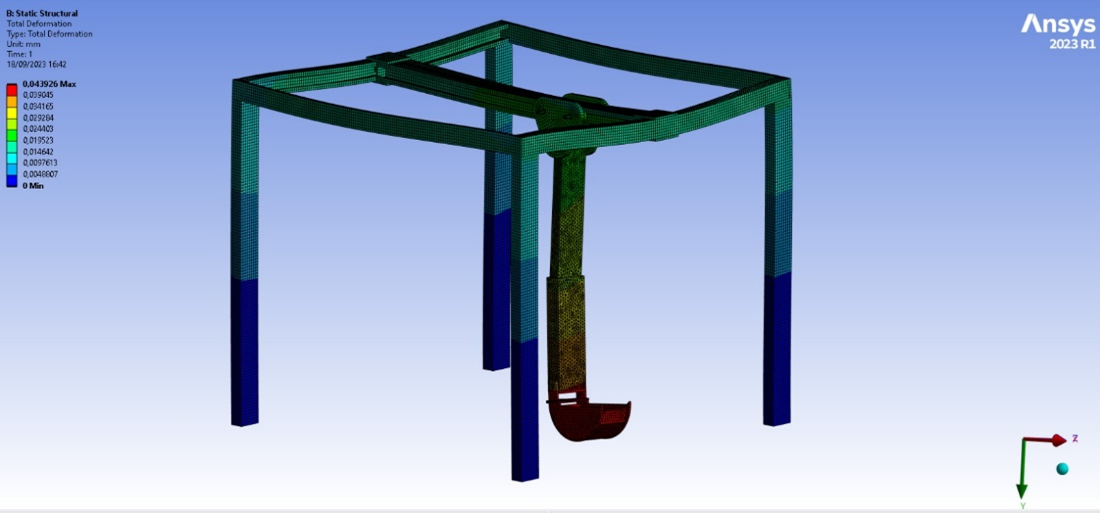
\includegraphics[width=1\linewidth]{Imagens/Resultado_1.png}
    \smallcaption{Fonte: Autor}
    \label{fig:Resultado_1}
 \end{figure}
 
\begin{figure}[!htp]
  \centering
  \begin{minipage}{0.7\textwidth}
        \caption{Deformações Mínimas e Maximas}
        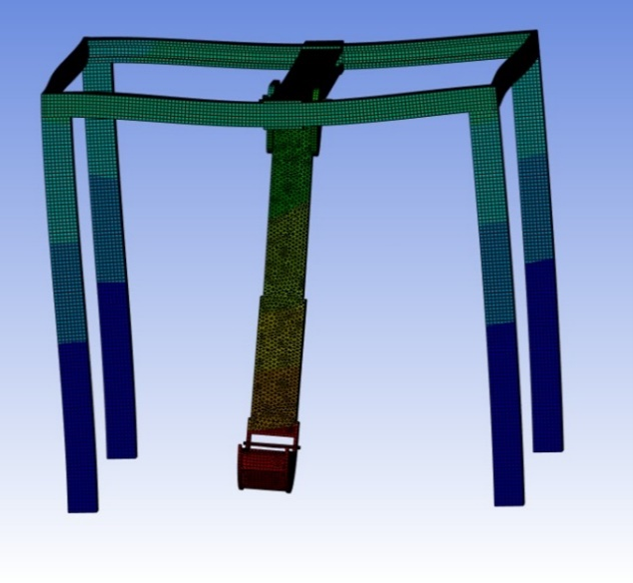
\includegraphics[width=0.6\linewidth]{Imagens/Resultado_2.png}
        \label{fig:Resultado_2}
  \end{minipage}
  \quad
  \begin{minipage}{0.7\textwidth}
        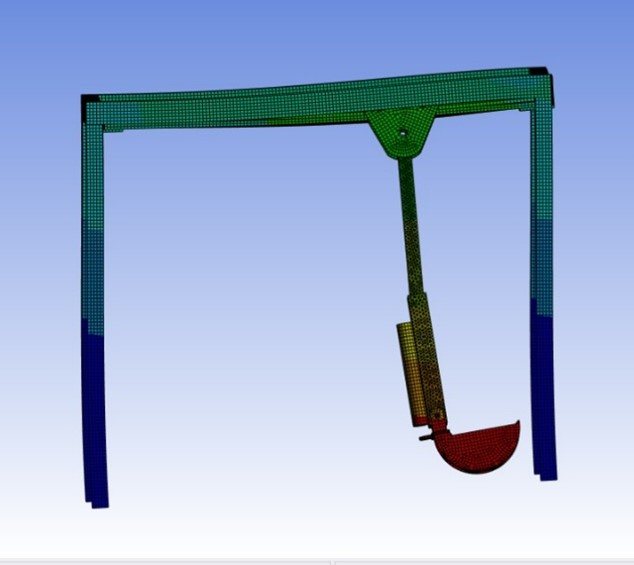
\includegraphics[width=0.6\linewidth]{Imagens/Resultado_3.jpg}
        \smallcaption{Autor}
  \end{minipage}
\end{figure}

\newpage

A Tensão equivalente Von-Mises, os valores máximos e mínimos obtidos, assim como a unidade utilizada estão indicados na Figura [\ref{fig:Vonmisses}] .

\begin{figure}[!htp]
 \centering
    \caption{Tensão equivalente Von-Mises}
    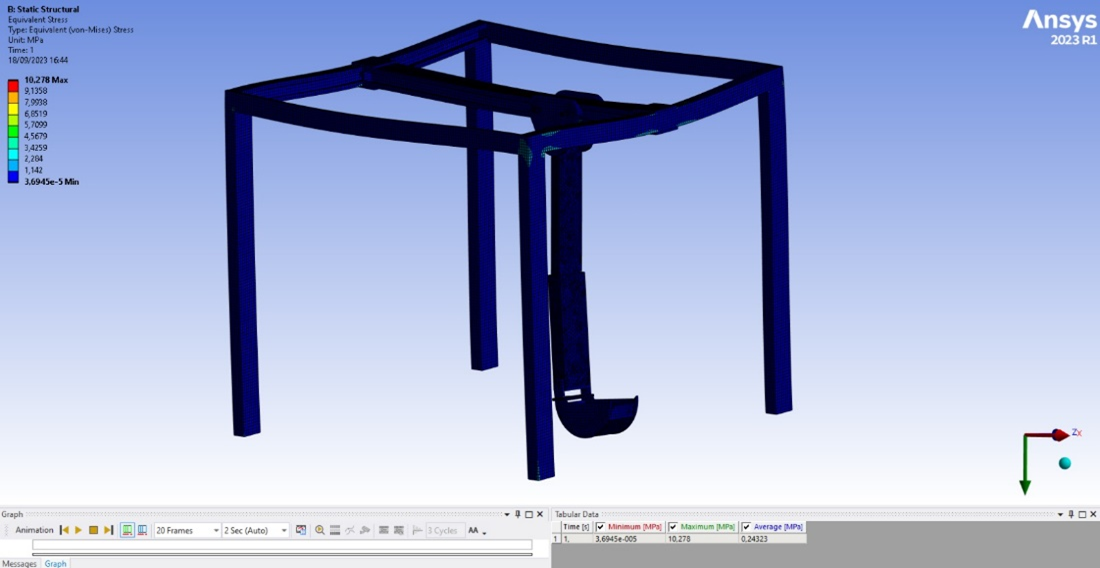
\includegraphics[width=1\linewidth]{Imagens/Vonmisses.png}
    \smallcaption{Fonte: Autor}
    \label{fig:Vonmisses}
 \end{figure}
 
\newpage

O “Strain energy”, a qual seria uma espécie de energia potencial acumulada em uma determinada parte da estrutura, como resultado de uma deformação elástica. Os valores máximos e mínimos obtidos, assim como a unidade utilizada estão indicados na Figura [\ref{fig:Maximo}].

\begin{figure}[!htb]
 \centering
    \caption{Strain energy}
    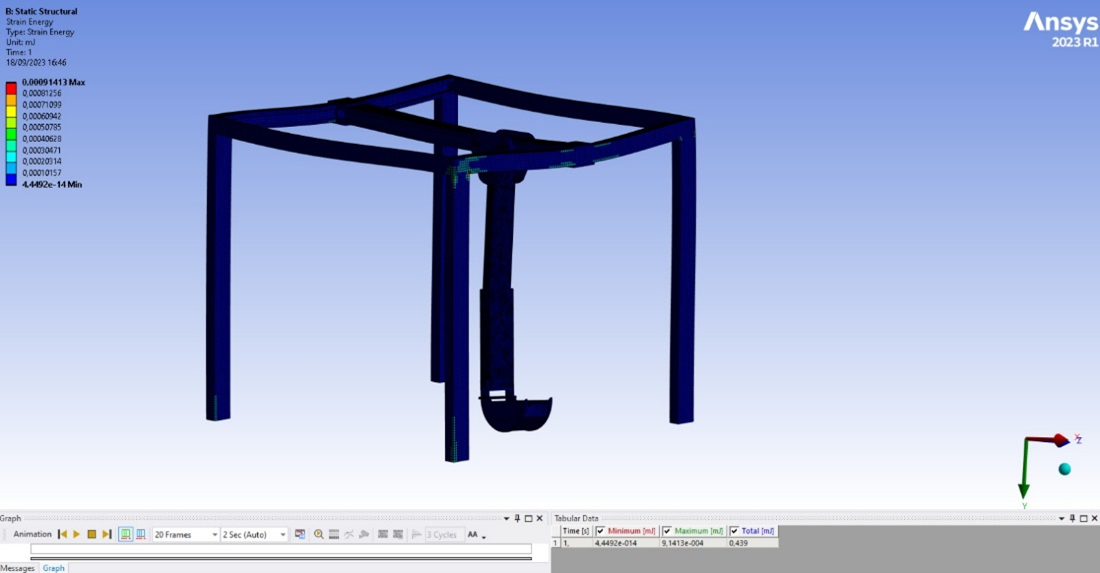
\includegraphics[width=1\linewidth]{Imagens/Maximo.png}
    \smallcaption{Fonte: Autor}
    \label{fig:Maximo}
 \end{figure}
 
\newpage

\chapter{Sistema de controle do modelo} 

Para o sistema de controle do modelo, foi pensado na implementação de motores elétricos, como o exemplificado na Figura \ref{fig:motor}, responsáveis por comandar o movimento da garra ao longo do trilho e o do próprio trilho. Dessa maneira, os motores seriam associados a polias que contenham o fio de nylon e, ao passo que o motor rotacione, o fio seria tensionado, promovendo a movimentação desejada. Vale ressaltar a existência de dois motores para cada movimento a fim de permitir o deslocamento para ambos os lados. Assim, a existência de sensores fim de curso nas extremidades de cada direção de movimento interroperiam o acionamento do motor, indicando um limite de deslocamento e impedindo avaria da estrutura.

\begin{figure}[!htb]
 \centering
    \caption{Exemplo de DC Brushless Motor}
    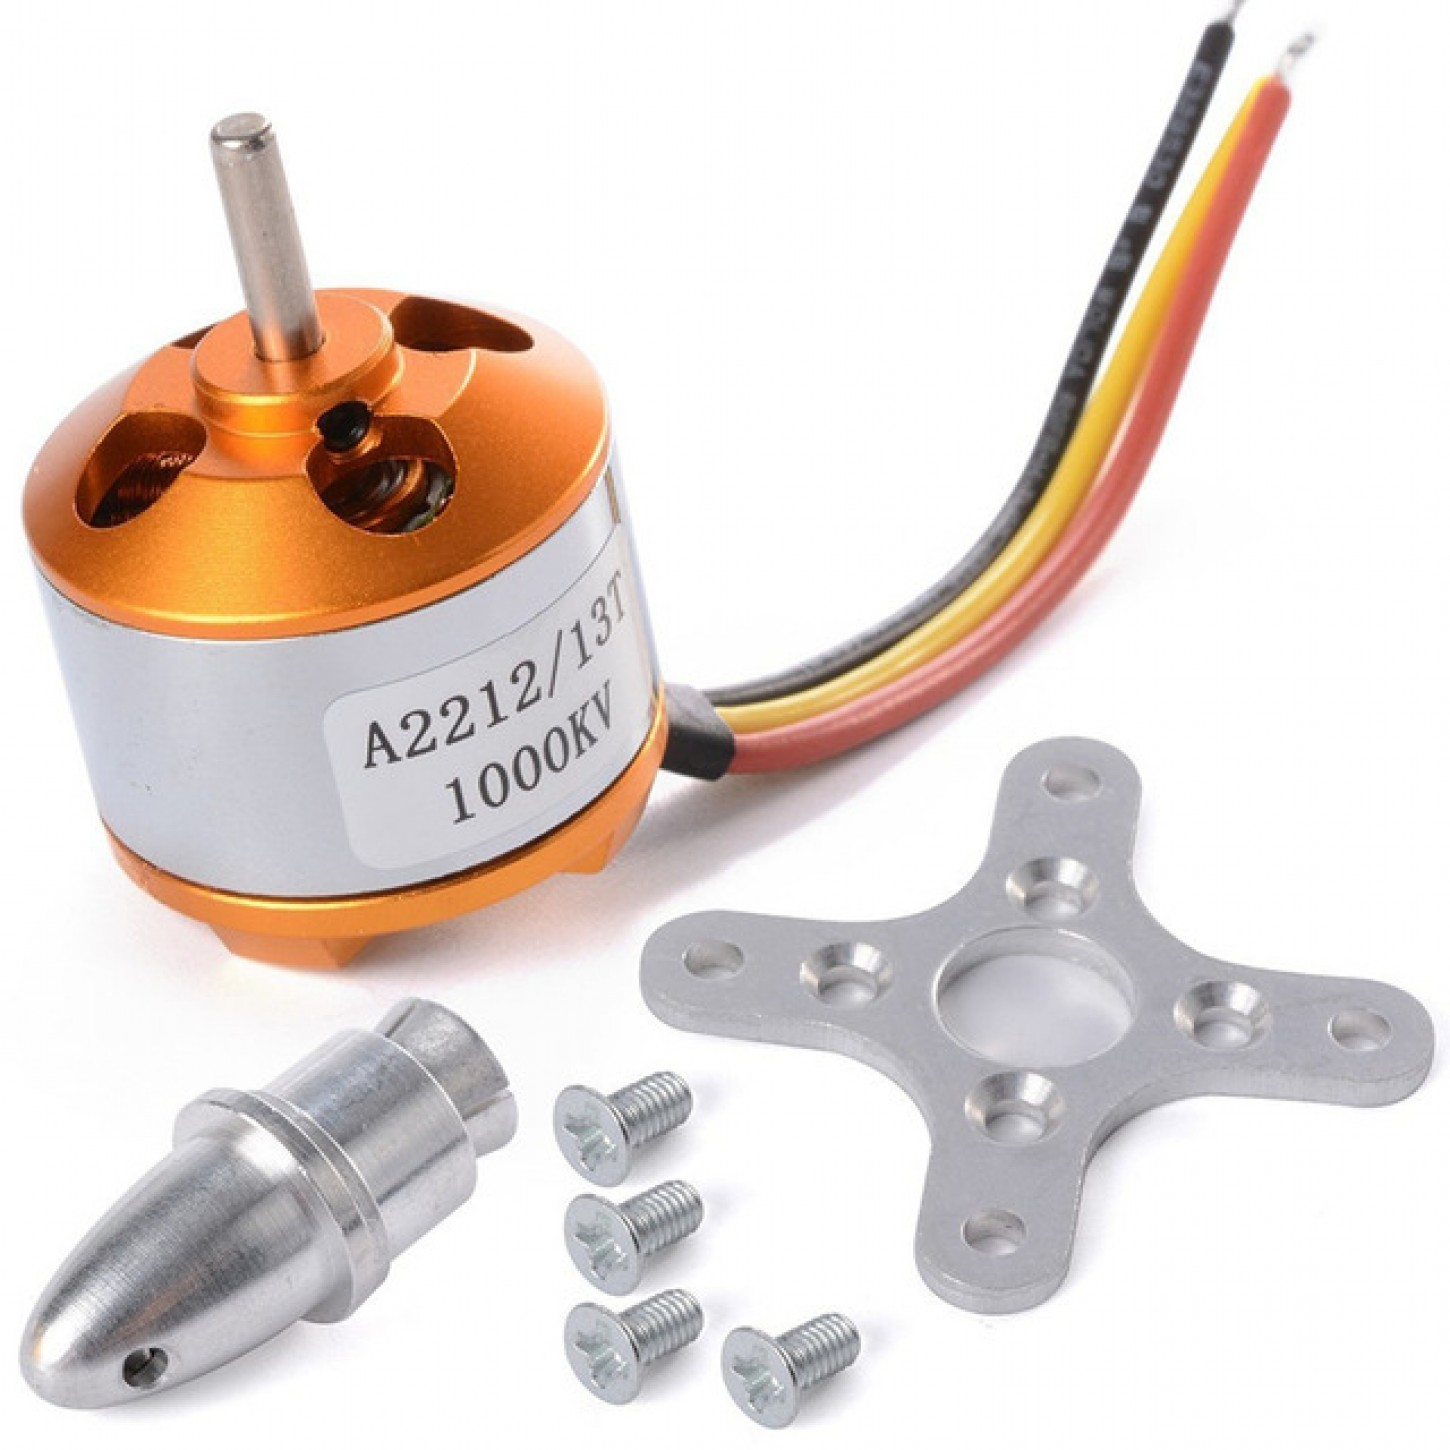
\includegraphics[width=0.5\linewidth]{Imagens/MOTOR A2212 F1-1450x1450.jpg}
    \smallcaption{Fonte: \textcite{motor}}
    \label{fig:motor}
 \end{figure}


Em relação ao movimento de subida e descida da garra, pensou-se novamente na implementação de um motor elétrico. Entretanto, neste caso, seria necessário apenas uma unidade, a qual rotacionaria em um sentido para promover a descida da garra e no sentido contrário para subir a mesma. Dessa maneira, um sensor infravermelho presente na extremidade da pá identificaria a distância da garra em relação ao solo, delimitando o movimento vertical dela. As Figuras \ref{fig:Fimdecurso} e \ref{fig:Infravermelho} indicam exemplos de sensores a serem utilizados no projeto

 \begin{figure}[!htp]
  \centering
  \begin{minipage}{0.4\textwidth}
    \centering
    \caption{Sensor Fim de Curso para Arduino}
    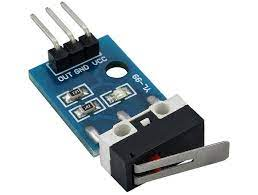
\includegraphics[width=1\linewidth]{Imagens/fim de cruso.jpg}
    \smallcaption{Fonte: \textcite{fimdecurso}}
    \label{fig:Fimdecurso}
  \end{minipage}
  \hfill
  \begin{minipage}{0.4\textwidth}
    \caption{Sensor Infravermelho para Arduino}
    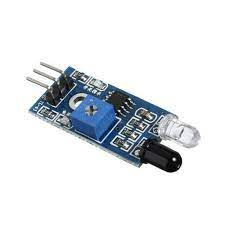
\includegraphics[width=1\linewidth]{Imagens/Infravermelho.jpg}
    \smallcaption{Fonte: \textcite{infravermelho}}
    \label{fig:Infravermelho}
  \end{minipage}
\end{figure}

\newpage

Por fim, para o movimento da pá, foi planejado um sistema eletropneumático, no qual contatos normalmente abertos fechariam com o acionamento de botoeiras, promovendo os deslocamentos da pá. Dessa maneira, os movimentos tanto dos motores quanto do sistema eletropneumático poderiam ser convertidos em uma lógica de programação carregada no Arduino, exemplificado na Figura \ref{fig:Uno} e assim, por meio de um módulo \textit{bluetooth} conectado a ele, seria possível o acionamento dos movimentos em um controle remoto, ou até, por um aplicatico no celular.

\begin{figure}[!htb]
 \centering
    \caption{Arduino UNO}
    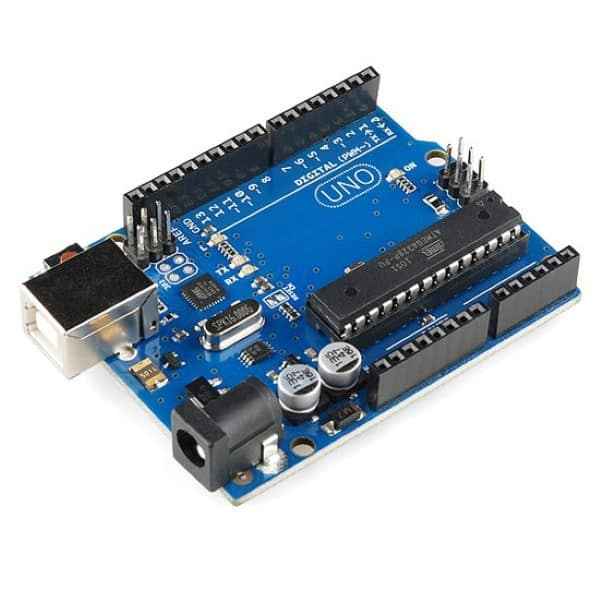
\includegraphics[width=0.5\linewidth]{Imagens/Uno.jpeg}
    \smallcaption{Fonte: \textcite{UNO}}
    \label{fig:Uno}
 \end{figure}

 Deste modo, o sistema de controle pensado para o modelo seria capaz de acionar e movimentar a estrutura remotamente, sendo possível o desenvolvimento de um aplicativo que consiga juntar todos os comandos e que seja apresentado ao usuário de forma simples e interativa, como um controle de \textit{videogame}.

\chapter{Cronograma atualizado do projeto}

 \begin{figure}[!htb]
 \centering
    \caption{Calendário}
    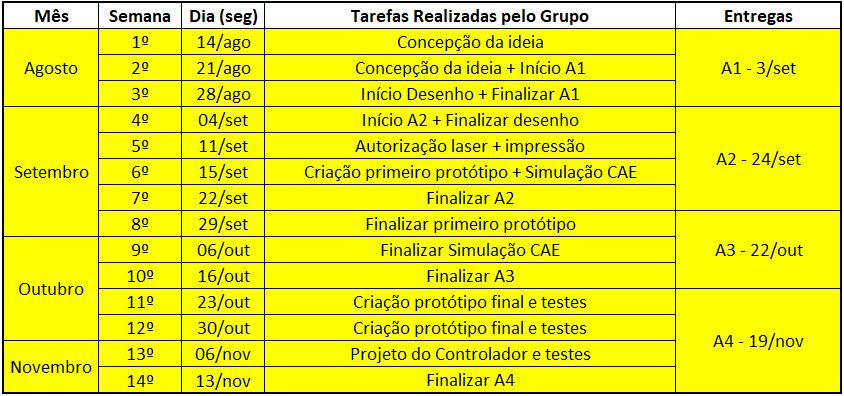
\includegraphics[width=1\linewidth]{Imagens/Cronograma.png}
    \smallcaption{Fonte: Autor}
    \label{fig:Calendario}
 \end{figure}

\chapter{Conclusões}

Com a montagem do protótipo feita, o grupo pode finalmente iniciar os testes e correções adequadas para que o projeto estivesse de acordo com o requerido. Após alguns ajuste pontuais, o projeto estava totalmente funcional, conforme demonstrado no \textit{link} do vídeo disponibilizado anteriormente. Dessa maneira, uma sugestão para um próximo projeto seria a implementação do sistema de controle do modelo, utilizando-se recursos físicos e testando-os  a fim de aprimorar o projeto inicial de acionamento manual.

\printbibliography
\nocite{*}

\end{document}